\documentclass[12pt]{article}

\usepackage{appendix}
\usepackage{comment}
\usepackage{mathtools}
\usepackage{fancyvrb}
\usepackage{cite}
\usepackage{paralist}
\usepackage[compact]{titlesec}
\usepackage{enumitem}
\usepackage{caption}
\usepackage[normalem]{ulem}
\usepackage{amsmath}
\usepackage{bbm}
\usepackage{amsthm}
\usepackage{thmtools, thm-restate}
\usepackage{mathrsfs}
\usepackage{amssymb}
\usepackage{tikz}
\usepackage{dsfont}
\usepackage{capt-of}
\usepackage{algorithmicx}
\usepackage{algorithm}
\usepackage[noend]{algpseudocode}
\usepackage[makeroom]{cancel}
\usepackage{datetime}
\usepackage[hang]{footmisc}

\newcommand{\codefalse}{\texttt{false}}
\newcommand{\codetrue}{\texttt{true}}
\newcommand{\codeedges}{\mathit{edges}}
\newcommand{\codedata}{\mathit{data}}

\newtheorem{lemma}{Lemma}

\begin{document}

\title{Snowpack: Scalable BFT Sequencing}
\author{John Boyd\thanks{john@cargodog.dev}}
\maketitle

\begin{abstract}
  Transaction sequencing is the primary bottleneck of consensus protocols.
  Modular consensus protocols address this limitation by deferring transaction
  execution to other layers of the protocol stack, and optimizing for the
  process of reaching sequence agreement. The majority of such protocols are
  leader-based or have greater communication complexity, which limit their
  ability to scale to large validator sets.

  Avalanche consensus is noteworthy for its ability to scale horizontally, and
  accommodate large validator sets; however, it is not possible to apply
  Avalanche consensus in a modular execution stack. Avalanche peers are unable
  to agree on transaction sequence, and therefore its consensus rules require
  transaction execution to resolve conflict set preferences. Additionally,
  Avalanche's multicolor problem requires secondary processes to avoid liveness
  failure.

  This work proposes Snowpack, an adaptation of Avalanche consensus, which
  employs a novel solution to the multicolor problem and provides transaction
  sequence agreement. In addition to improving performance, this solution
  allows extraction of ordering constraints from a block DAG to build a
  constraint DAG. Ordering constraints form mutually exclusive conflict sets,
  and the resultant graph is compatible with Avalanche consensus. Peers are
  then able to reach agreement on the set of ordering constraints, from which
  they can derive the total block ordering.

  This design combines the horizontal scalability of Avalanche consensus with
  the performance benefits of modular execution. Snowpack has applications as a
  scalable decentralized sequencer for rollups or internet-scale decentralized
  applications.
\end{abstract}

\section{Introduction}
\subsection{Scaling and User Experience in Web3}
  The rise in popularity of decentralized applications has spurred research
  interest in techniques to improve their performance and user experience. As
  more users participate in a decentralized application, protocol validators
  are tasked with servicing an ever increasing volume of transactions. When a
  protocol reaches the limits of its transactional capacity, the decentralized
  applications hosted which rely on that protocol suffer. Sudden fee increases
  \cite{CryptoKitties, al2021cryptocurrency, katsiampa2019empirical,
  saef2023regime} or service outages \cite{SolanaRestart} are an unbearable
  inconvenience to many users, while unpredictable costs and user experiences
  deter developers.

  Modular protocol stacks with transaction execution separated from consensus,
  have seen a surge in popularity \cite{LazyLedger, avail}, due to their
  compatibility with vertical and horizontal scaling solutions. These protocols
  focus on applications which can be modeled as state-machine replication
  problems \cite{schneider1990}, optimizing the consenus protocol for
  transaction ordering, and leaving transaction execution to be performed by
  execution-optimized protocols higher in the protocol stack. Removing
  transaction execution from consensus greatly reduces latency in the agreement
  process, speeding process convergence towards consensus
  \cite{wan2019evaluating}. This allows developers to focus improving the
  vertical scalability of execution modules, while also facilitating horizontal
  scaling through the use of parallel execution modules.

  The prevailing challenge in modular protocol stacks, is finding the right
  balance of consistency and availability of state for a given application.
  Parallel execution modules require special care to enable state sharing for
  cross-module interactions. Futher complicating this, different applications
  may have different preferences. Some applications may prefer local-only state
  availability with maximum throughput, while others may be willing to
  compromise performance for greater interoperability with other applications.
  Attempts to enable safe state sharing across modules often compromise
  performance or lead to centralization.

\subsection{Horizontal Scaling Without Partitioning}
  The Avalanche consensus protocol is unique in its ability to reach byzantine
  agreement with only constant-sized communication \cite{rocket}. This allows
  horizontal scaling without network partitioning. New validators may join the
  protocol to increase the security and availability of the network without
  degrading network performance. Importantly, this is possible without
  partitioning validators into shards or L2s, sparing developers and users the
  interoperability challenges that would otherwise arise. Instead, capacity
  scales fluidly with the addition of new validators, similar to traditional
  web infrastructure.

  Despite Avalanche's ability to fluidly scale horizontally, it is not possible
  to remove transaction execution from the consensus protocol, preventing it
  from taking advantage of the performance benefits of modular protocols. This
  is a direct consequence of its DAG structure. Because blocks may be inserted
  simultaneously, there is no agreed upon block ordering. As a result,
  applications cannot rely on a simple ordering rule to pick a preferred
  transaction when conflicting transactions are detected. Instead transactions
  must be executed as part of the consensus protocol, so that peers may reach
  agreement on the preferred transaction in each conflict set.

\subsection{This Work}
  This work presents the Snowpack consensus protocol, an adaptation extension
  to Avalanche consensus which offers a unique solution to the multicolor
  problem. This solution further enables the ability to reach agreement on
  transaction ordering, without compromising Avalanche's constant-sized
  communication complexity. Snowpack also incorporates data availability
  sampling (DAS) \cite{albassam2019fraud} to minimize bandwidth requirements.

  A naive approach to improving the scalability of Avalanche might be to
  eliminate transaction execution from the consensus protocol, as in
  \cite{LazyLedger}. However, since Avalanche consensus does not provide
  transaction ordering, it would not be possible to safely replicate
  application state-machines in a Byzantine setting. As we explore in
  \ref{sec:State-machine Replication}, the final state after executing a
  deterministic state-machine depends on the order of transactions which get
  executed. A failure to agree on the transaction sequence would lead to
  potential byzantine faults.

  As such, Snowpack aims first to solve the problem of total ordering in
  Avalanche. Rather than employing the Snowman solution to the multicolor
  problem, which leads to performance limitations \cite{buchwald2024frosty},
  Snowpack proposes a novel solution to the multicolor problem, by solving a
  system of ordering constraints. Snowpack blocks encode partial ordering
  constraints, which are extracted to form a constraint graph. These
  constraints are mutually exclusive, and thus form binary conflict sets which
  guarantee process convergence. Once peers agree on a preferred set of partial
  ordering constraints, they may deterministically derive the total block
  ordering with no additional communication.

  Snowpack offers an improved performance over the Snowman adaptations of
  Avalanche consensus. With the added sequence agreement, Snowpack is further
  useful as a decentralized sequencer. It may be used as a decentralized
  alternative to the centralized sequencers currently employed by many L2s
  today. Ultimately, thanks to its sequencing guarantees, transaction execution
  may be eliminated from consensus, enabling new protocols with horizontal and
  vertical scaling of both consensus and transaction execution, suitable for
  internet-scale decentralized applications.

\section{Background}
\subsection{State-machine Replication}
  \label{sec:State-machine Replication}
  Decentralized applications can be modeled as replicated state-machines. In
  this model, a dynamic group of participants independently attempt to
  replicate the state of an application, by executing transactions with
  identical copies of the application state-machine. Any deterministic
  state-machine may safely be replicated, so long as peers can agree on the
  correct sequence of transactions to execute. The problem of ensuring peers
  agree on the application state is known as the state-machine replication
  (SMR) problem \cite{schneider1990}.

  Bitcoin offered the first practical decentralized replicated state-machine
  \cite{naka}. While Bitcoin's blockchain was specifically designed for a
  peer-to-peer cash application, subsequent smart-contract execution protocols
  such as \cite{buterin2014ethereum, SolanaWhitepaper} have gained popularity
  for their use as a general solution for a wide array of applications. These
  protocols are considered monolithic, because the full suite of application
  requirements (sequencing, execution, storage, etc) are all solved as part of
  the consensus protocol. Due to the performance limitations of monolithic
  designs, many have turned their attention to modular protocol stacks as a
  means to achieve internet-scale decentralized applications \cite{LazyLedger,
  avail}.

  The SMR model is the foundation upon which protocol modularization can occur.
  Modularization allows for sequencing, transaction execution, distributed
  storage, or any other feature a decentralized application requires, to be
  handled in its own protocol and composed into an application protocol stack. 
  
  As long as peers are able to agree on the set and sequence of transactions,
  these protocols may be composed to meet the needs of any decentralized
  application. Because decentralized sequence agreement can only be achieved
  through consensus, decentralized sequencers make a natural base layer for a
  modular protocol stack. For this reason, much attention has been given to the
  development of scalable sequencing protocols \cite{astriaIntro,
  espressoIntro}.

\subsection{Avalanche Consensus}
\subsubsection{Overview}
  Rocket et al. introduced Avalanche as the latest in a collection of
  probabilistic and leaderless consensus protocols\cite{rocket}. These
  protocols make novel use of network sampling to create a metastable mechanism
  which drives network participants to quickly converge on a decision for every
  transaction. Thanks to the constant-sized communication complexity of the
  sampling process, their design is able to scale horizontally to large
  validator sets. The addition of new validators increases the network's
  capacity for users, while the total transactional throughput is limited to
  the vertical scaling limits of those validators. As a result, Avalanche
  protocols are able to sustain high transactional throughput without
  compromising decentralization.

\subsubsection{Construction}
  The Avalanche protocol records transactions into a DAG. As transactions
  disseminate across the network, nodes will insert them into the DAG and group
  transactions into conflict sets. Each peer then queries a randomly selected,
  constant-sized subset of its peers for their preferred transaction in each
  conflict set. Once a node determines his peers' preference for a transaction.
  Each preferred transaction receives a chit, and accumulates a confidence
  score computed as the weight of the chits in its progeny. Once a transaction
  reaches the threshold confidence, it is considered final and written into the
  transaction database.

  A node's preference for a transaction may change, even after the initial
  insertion and query process, if queries for subsequent transactions indicate
  that the transaction is no longer connected to the most preferred graph. This
  rule to adopt the preference of his peers is what makes indecision a
  metastable condition and drives peers to converge on one common decision.

\subsubsection{Multicolor Problem}
  \label{sec:Multicolor Problem}
  The Avalanche consensus protocol can be modeled as a graph coloring process
  over the graph of transaction conflict sets. Each conflict set is a vertex in
  the graph, and peers assign a color to each, representing the preferred
  transaction within that set. Consensus is achieved when all peers agree on
  the color of a given vertex. Initially peers randomly assign a color to each
  vertex. As the process progresses, peers will adopt each other's color
  preferences. If the process converges, all peers will unanimously agree on
  the color assigned to each vertex in the graph.

  The multi-color problem arises as transaction conflicts increase. In
  practice, transactions may have arbitrarily many conflicts, and such each
  conflict set may have arbitrarily many possible colors As described in
  \cite{buchwald2024frosty}, the probability of the process converging
  decreases as the probability of two peers initially assigning the same color
  to a given vertex decreases. Thus, for applications where transaction
  conflicts are unbounded, the multi-coloring problem can lead to a liveness
  failure for any such vertex.

  For a two-colored graph, randomness of the Avalanche sampling process causes
  disagreement to be a metastable condition. In expectation, the process will
  make progress with each iteration and eventually converge. This is not the
  case for a multi-color graph. If we assume colors are assigned uniformly at
  random, then the probability of convergence decreases toward zero as the
  number of possible colors increases. This is known as the multi-color
  problem, and poses a challenge to applications whose transactions do not form
  binary conflict sets.

  The Avalanche authors propose Snowman consensus as a solution to this
  multi-coloring problem \cite{buchwald2024frosty}. Snowman performs a binary
  decomposition of each multi-colored conflict set into $log_2(L)$ two-colored
  subsets, where $L$ is the size of the multi-colored set. Snowman then
  sequentially executes Avalanche consensus on each subset, and because each
  subset is a binary choice, Avalanche is guaranteed to converge on a
  preference for each. Finally, the preference in each of the subsets form a
  path to exactly one block to be preferred in the original multi-colored
  conflict set.

  While Snowman guarantees process convergence, it greatly slows the time to
  convergence due to the need to execute multiple sequential Avalanche
  processes. The authors suggest the use of elected proposers to reduce the
  probability that two proposers may submit blocks simultaneously. This
  practically eliminates multi-colored conflict sets, so that only a single
  instance of Avalanche consensus needs to be executed for each block; however
  this effectively reduces the DAG to a simple blockchain, losing the
  performance benefits of a DAG.

\subsection{Data Availability Sampling}
  Al-Bassam et al. introduced the concept of data availability sampling (DAS)
  \cite{albassam2019fraud}, as a mechanism to reduce the communication
  requirements of peers in a peer-to-peer network. DAS makes use of erasure
  codes and random sampling to provide a statistical guarantee of data
  availability without requiring all peers to fully replicate all data. Use of
  DAS enables protocols to scale horizontally, allowing peers to share in data
  replication as more peers join the network.

  Erasure codes enable recovery of missing data, with only a subset of the data
  \cite{peterson1972error}. Any message $m$ may be erasure-coded, whereby the
  message is encoded into larger message $m'$ consisting of $k$ message shares,
  with the property that only $n < k$ shares are required to reconstruct $m$.
  The ratio of $\frac{n}{k}$ is referred to as the code rate, and is determined
  by the erasure-coding scheme. Perhaps the most widely studied erasure codes
  are Reed-Solomon codes, which can support a code rate of $\frac{1}{2}$
  \cite{reedsolomon}. Adaptations of Reed-Solomon codes have been proposed with
  various performance tradeoffs \cite{dudek, saints, shea, wu}.

  Al-Bassam et al. propose the use of two-dimensional erasure codes. This, in
  combination with the use of fraud proofs, enables peers to get strong
  statistical guarantees of data availability, importantly without needing to
  download all the data. First, every message on the network must commit to a
  merkle root of the full list of erasure codes. Before accepting any data into
  the data availability network, participants must be able to recover one row
  of the two-dimensional encoding. To prevent bad actors from submitting
  incorrectly coded data (e.g. to attempt a withholding attack), any
  participant which discovers an invalid row of the two-dimensional structure
  must broadcast fraud proofs to his peers.

  The robustness of this scheme depends on the number of samples taken and the
  number of rows in the two-dimensional codes. Dividing the code data across
  more rows reduces the amount of data each participant must download, but
  increases the number of samples required to have certainty in detecting a
  fraudulently coded row. Since the number of samples taken relates to the
  number of network participants, then, by extension, the robustness of this
  scheme depends on the number of network participants.

\section{Snowpack: Scalable BFT Sequencing}
\subsection{Network Model}
  The network model used is comprised of the following types of participants:

  \begin{itemize}
    \item \textbf{Validator nodes.} These nodes participate in consensus to
      decide which blocks should be accepted into the block DAG.
    \item \textbf{Client nodes.} These nodes provide end users with access to
      the network. They accept and submit user transactions to the network, and
      provide users with the network state necessary to interact with
      decentralized applications.
  \end{itemize}

  Snowpack transactions are serialized into blocks, which form the vertices in
  the block DAG. Each block references multiple parents and commits to the
  preferred order of those parents. Blocks are accepted into the DAG regardless
  of transaction contents. In fact, there is no notion of transaction validity
  in the Snowpack protocol.

  Similar to Avalanche, Snowpack treats the Sybil problem as separate from that
  of consensus \cite{rocket}. Validators are expected to employ some sybil
  control mechanism, such as proof-of-work or proof-of-stake, but Snowpack
  implementations have freedom to choose the mechanism which provides the best
  incentives for a given use case.

  Validators and gateways both participate in the gossip messaging network. The
  gossip network is responsible for disseminating transactions and blocks as
  users and validators, respectively, propose them.

\subsection{Goals}
  Snowpack has the following design goals:

\begin{enumerate}
  \item \textbf{Availability-only block validity.} A block should be considered
    valid if the transaction data it references is available to the network.
    Nodes do not need to execute transactions to assert block validity.
    \label{goal:availability}
  \item \textbf{Sequence agreement.} Network participants must converge
    on one common understanding of the total ordering of transactions.
    \label{goal:agreement}
  \item \textbf{Horizontal Scalability.} The addition of validators should increase the
    network's capacity for users and user transactions.
    \label{goal:scalability}
\end{enumerate}

\subsection{Notation and Terminology}
  This work makes use of two DAGs: a graph of blocks referred to as block DAG,
  and a graph of ordering constraints referred to as the constraint DAG. Blocks
  form the vertices of the block DAG, and ordering constraints form the
  vertices of the constraint DAG.

  Blocks are annotated according to their height $h$ in the block DAG and order
  of observation $i$, as $b_{h,i}$. For example, the first block we observe at
  height 9 would be denoted as $b_{9,0}$.

  Ordering constraints are denoted as $[b_a, b_b]$, where $b_a$ is constrained
  to have been observed before $b_b$. Constraints may be referred to as $c_{h,i,n}$, which
  represents the $n^{th}$ constraint of block $b_{h,i}$.

  A special case exists for blocks which only reference one parent, which we
  refer to as the empty constraint: $[b_a, -]$. The empty constraint does not
  actually constrain the ordering of block $b_a$ relative to any other block.
  It exists only to assist connectivity of the constraint DAG.

\subsection{Solving The Multi-coloring Problem}
  As discussed in \ref{sec:Multicolor Problem}, Avalanche is susceptible to a
  multi-coloring problem. It is not guaranteed to converge for graphs whose
  transactions are members of multi-colored conflict sets. While solutions for
  the multi-coloring problem exist \cite{buchwald2024frosty}, this work
  improves on those by eliminating the need to execute sequential instances of
  Avalanche, while also achieving total ordering, and without reducing the DAG
  to a simple blockchain.

  Similar to \cite{buchwald2024frosty}, this work partitions multi-colored
  conflict sets into two-colored subsets. We accomplish this by extracting
  parent-ordering constraints from each block, instead of performing a binary
  decomposition of the conflict set. Ordering constraints reference each other
  and form the constraint DAG. Because ordering constraints only conflict with
  their opposite, i.e. $[p_0, p_1]$ can only conflict with the constraint
  $[p_1, p_0]$, the maximum size of a conflict set in the constraint DAG is 2
  (two-colored). Given this, Avalanche consensus is guaranteed to converge when
  executed on the constraint DAG.

  Consensus is reached on the constraint DAG by executing Avalanche on the
  constraint conflict sets, to decide the preferred constraint set. Once every
  constraint committed to by a particular block has been accepted into the
  constraint DAG, that block is inferred to be accepted into the block DAG
  without any consensus process on that DAG. In this way, Snowpack inherits the
  properties of Avalanche consensus, namely its horizontal scalability, safety,
  and liveness properties, satisfying the corresponding Goal
  \ref{goal:scalability}. While this does require multiple instances of
  Avalanche to be executed for a given block, each instance may be executed
  concurrently rather than sequentially. Compared to \cite{buchwald2024frosty}, this
  construction allows Snowpack to reach agreement in the same time as standard
  Avalanche consensus, at the cost of increased communication.

\subsection{Constructing the Constraint DAG}
  Each block commits to a list of ordering constraints, as determined by the
  list of parent blocks it references. A block will commit to the empty
  constraint for each of its parents, as well as the partial ordering
  constraints for every combination of pairs of its parents, which do not
  violate the block's stated parent sequence. For example, consider some block
  $b_{h,i}$ which lists parents $p_0$, $p_1$, and $p_2$ in that order. Block
  $b_{h,i}$ would commit to the following constraints: $[p_0, -]$, $[p_1, -]$,
  $[p_2, -]$, $[p_0, p_1]$, $[p_0, p_2]$, $[p_1, p_2]$. Each constraint
  implicitly depends on the parent blocks it references. These dependencies
  form the edges of the constraint DAG.

  Figure \ref{fig:block_dag} illustrates an example block DAG, with blocks
  $b_{2,0}$ and $b_{2,1}$ in conflict due to their conflicting parent
  orderings. Figure \ref{fig:block_dag_with_constraints} expands the example
  DAG to illustrate the parent ordering constraints of each block. Figure
  \ref{fig:constraint_dag} illustrates the constraint DAG constructed from the
  constraints in this example. Duplicate constraints are eliminated.

  \begin{figure}
    \centering
    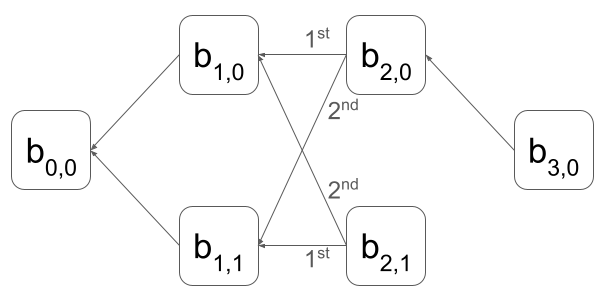
\includegraphics[width=\columnwidth]{images/block_dag.png}
    \caption{Illustration of a block DAG. Blocks $b_{2,0}$ and $b_{2,1}$ indicate
      which parents they observed first. Notice they each observed blocks
      $b_{1,0}$ and $b_{1,1}$ as parents, but in opposing
      order.}\label{fig:block_dag}
  \end{figure}

  \begin{figure}
    \centering
    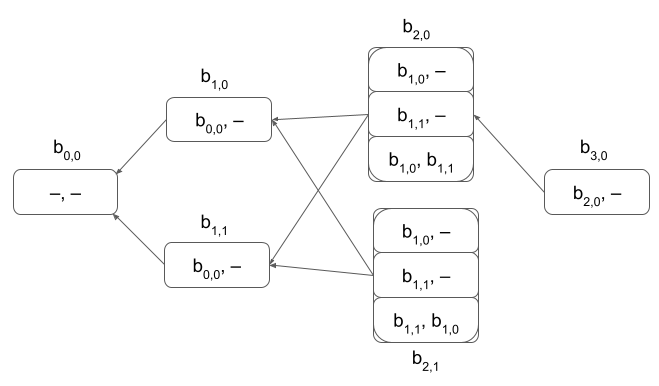
\includegraphics[width=\columnwidth]{images/block_dag_with_constraints.png}
    \caption{Expanded block view, showing the parent ordering constraints of
      each block, for the block DAG given in Figure \ref{fig:block_dag}.
      }\label{fig:block_dag_with_constraints}
  \end{figure}

  In order to use Avalanche consensus to reach agreement on the constraint DAG,
  we must define how conflict sets are grouped. As mentioned earlier, ordering
  constraints are binary, and may only conflict with their opposite.
  Additionally, in order to satisfy Goal \ref{goal:availability}, no other
  block or transaction data will be evaluated, and thus will not impact the
  formation of conflict sets. To determine if two constraints $[a, b]$ and $[c,
  d]$ conflict, we need only test if $a = d$ and $b = c$. Figure
  \ref{fig:constraint_dag} illustrates the conflict sets as dashed lines around
  each constraint in the constraint DAG. Constraints with no conflicts become
  the only members of singleton conflict sets. Constraints $[b_{1,0}, b_{1,1}]$
  and $[b_{1,1}, b_{1,0}]$, however, are members of the same conflict set,
  because they reference their parent blocks $b_{1,0}$ and $b_{1,1}$ in
  opposing order. Avalanche consensus will resolve the preferred constraint in
  each conflict set.

  \begin{figure}
    \centering
    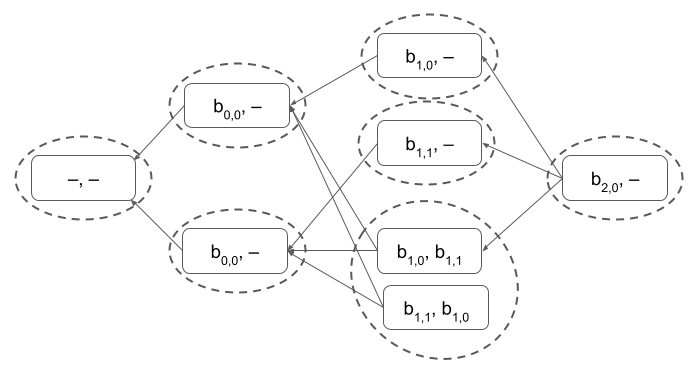
\includegraphics[width=\columnwidth]{images/constraint_dag.png}
    \caption{Illustration of the constraint DAG, constructed from the
      constraints from the blocks in Figure
      \ref{fig:block_dag_with_constraints}. Conflict sets are indicated by
      dashed lines.
      }\label{fig:constraint_dag}
  \end{figure}

\subsection{Determining Block Sequence}
  As parent ordering constraints are accepted into the constraint DAG, it
  becomes possible to ascribe a final sequence to the blocks in the block DAG.
  Once every constraint referencing any block in the progeny of block $b$ has
  been accepted, the sequence of blocks leading up to $b$ may be computed
  recursively by merging the sequence at each parent, eliminating duplicates,
  and appending each parent in order to the sequence, as given in
  Figure \ref{alg:sequencing}.

  \begin{figure}
  \begin{center}
  \small
  \begin{algorithmic}[1]
      \Procedure{sequenceAt}{$b$}
        \State $\mathcal{S} := \emptyset$
        \For{$b' \in \mathcal{B}: b' \stackrel{*}{\gets} b$}
          \For{$b'' \in \mathcal{B}: b'' \in \Call{sequenceAt}{b'} \land b'' \notin \mathcal{S}$}
            \State $\mathcal{S} = \mathcal{S} || b''$
          \EndFor
        \EndFor
        \For{$b' \in \mathcal{B}: b' \stackrel{*}{\gets} b$}
            \State $\mathcal{S} = \mathcal{S} || b'$
        \EndFor
        \State \Return $\mathcal{S}$
      \EndProcedure
      \captionof{figure}{Algorithm to determine sequence of events preceding a
      given vertex.} \label{alg:sequencing}
  \end{algorithmic}
  \end{center}
  \end{figure}

  If two blocks disagree in the order of observation of their parents, they
  will produce conflicting parent ordering constraints. Eventually, one of the
  conflicting constraints will become rejected from the constraint DAG, at
  which point the block will be considered rejected from the block DAG. This
  ensures that peers will not only agree on the set of blocks, but the sequence
  of blocks, thereby satisfying \ref{goal:agreement}.

  When executing this sequencing algorithm on the example DAG in Figure
  \ref{fig:block_dag}, to determine the sequence at $b_{3,0}$, we arrive at the
  following sequence: $b_{0,0}$, $b_{1,0}$, $b_{1,1}$, $b_{2,0}$, $b_{3,0}$.

\subsection{Data Availability Criteria}
  To improve the scalability of the network, this work employs data
  availability sampling, as described by Al-Bassam et al.
  \cite{albassam2019fraud}. This enables peers to ensure all requisite data
  exists and is available to those who need it, without requiring every peer to
  download and retransmit all block data. Enabled by the fact that transaction
  validity is not a criteria for block acceptance, this accomplishes
  Goal \ref{goal:availability}.

  Before considering a block for acceptance, a node must sample $i$ consensus
  peers for a proof of data availability for the block data. $i$ as well as the
  error-correction scheme used should be selected according to
  \cite{albassam2019fraud}, in order to achieve the desired certainty of data
  availability. The bandwidth required for these data-availability checks is
  $O(\sqrt{s}+log{\sqrt{s}})$ for each challenge, where $s$ is the size of the
  block data.

  Additionally, upon detecting an invalid erasure code, a fraud proof must be
  relayed to peers so that they may verify the fraud. Upon verifying fraudulent
  behavior, the network should penalize the offending peer. The exact penalty
  is outside the scope of this paper, and may take the form of stake slashing
  if proof-of-stake is employed, or some other economic penalty.

\subsection{Safety}
  Snowpack inherits the safety assumptions of the data-availability proofs
  described in \cite{albassam2019fraud}, as well as the Avalanche protocol
  described in \cite{rocket}. Al-Bassam et al. show that their construction of
  data availability proofs can only be considered secure when $(k+1)^2$ samples
  are taken. Since the number of samples taken is a function of the number of
  peers in the network, we recommend each peer dynamically select $i$ based on
  the number of consensus nodes he observes. Precisely, each peer should choose
  $i$ according to Eq.(\ref{func:choose_i}).
  \begin{equation}\label{func:choose_i}
    i = \min(1, \frac{(k+1)^2}{\#peers})
  \end{equation}

  Rocket et al. shows that Avalanche consensus is secure against Byzantine
  faults for any adversarial presence of $ 0 <= f' <=
  \frac{n(k-\alpha-\Psi)}{k} <= f $ where $f'$ is the number of adversarial
  peers in $f$, and $n, k, \alpha, \Psi$ are protocol parameters.

\section{Conclusion}
  This work introduces a novel BFT sequencing protocol. The core innovation is
  the protocol's use of partial ordering constraints and Avalanche consensus to
  reach agreement on the total order of blocks in a block DAG, without
  compromising the scalability properties of Avalanche. By achieving total
  ordering, Snowpack is compatible with modular scaling techniques, enabling it
  to serve as a horizontally scalable foundation for a modular protocol stack.

  Snowpack may be applied as a performance improvement to existing
  Avalanche-based protocols. Other applications include decentralized shared
  sequencing for L2s, or new smart-contracting systems aiming for horizontal
  scalability and modularity.

\bibliographystyle{plain}
\bibliography{paper}

\end{document} 
